\documentclass[xetex,aspectratio=43]{beamer}

\usepackage{res/lections}

\preamble

\title{Примеры архитектур: Intel x86 и RISC-V}

\begin{document}

    \titleslide

    \tocslide


%==============================================

\section{Архитектура и система команд x86}

\subsection{Регистры и адресация}

\begin{frame}{Регистровый файл (1)}
        Регистры (для 32-битной ЭВМ)

        \begin{itemize}
            \tightlist
            \item
            EAX (общий, аккумулятор), EDX (умножение и деление вместе с EAX), EBX
            (указатели), ECX (счетчик)
            \item
            EDI (dest index), ESI (source index)
            \item
            EBP, ESP, EIP
            \item
            CS, SS, DS, ES, FS, GS --- сегментные
            \item
            EFLAGS
        \end{itemize}

        \pause

        Фрагменты регистров

        \begin{itemize}
            \tightlist
            \item
            \_H, \_L --- 8-разрядные
            \item
            \_X, \_S --- 16-разрядные
            \item
            E\_ --- 32-разрядные
            \item
            R\_ --- 64-разрядные
        \end{itemize}

        Например, для аккумулятора

        (AH (8), AL (8)) $\rightarrow$ AX (16) $\rightarrow$ EAX (32) $\rightarrow$ RAX (64)
\end{frame}

\begin{frame}{Регистровый файл (2): EFLAGS}
Регистр флагов EFLAGS.
    Весь регистр 32-битный (начиная с 80386).

    Основные флаги (с 8086):

    \begin{itemize}
        \tightlist
        \item
        OF --- флаг переполнения
        \item
        DF --- флаг направления
        \item
        IF --- флаг прерывания
        \item
        TF --- флаг трассировки
        \item
        SF --- флаг знака
        \item
        ZF --- флаг нуля
        \item
        AF --- флаг дополнительного переноса (для упакованных
        двоично-десятичных операций)
        \item
        PF --- флаг четности
        \item
        CF --- флаг переноса
    \end{itemize}
\end{frame}

\begin{frame}{Адресация данных}
    \begin{itemize}
        \item
        Непосредственная (аргументы в коде)
        \item
        Регистровая (номер регистра в коде)
        \item
        Память{[}E\_X + смещение{]}, Память{[}EBP + смещение{]}, + возможно
        префиксы сегментов
    \end{itemize}
\end{frame}

\subsection{Система команд}

\begin{frame}{Команды пересылки данных}
    \begin{itemize}
        \tightlist
        \item
        MOV память обменивается только с арифметическими регистрами, ESI, EDI
        \item
        XCHG reg, mem/reg
        \item
        LAHF, SAHF --- флаги \(\leftrightarrow\) AH
    \end{itemize}
\end{frame}

\begin{frame}{Команды АЛУ}
    \begin{block}{Логические}
        AND, OR, XOR, NOT
    \end{block}

    \begin{block}{Арифметические}
        \begin{itemize}
            \item
            ADD, SUB, ADC, SBB, INC, DEC, NEG
            \item
            MUL (reg/mem), DIV (reg/mem), IMUL, IDIV,
            \item
            CWQ (EAX \(\rightarrow\) EDX:EAX)
        \end{itemize}
    \end{block}

    \begin{block}{Сдвига}
        \begin{itemize}
            \item
            ROR, ROL
            \item
            RCL, RCR --- с переносом
            \item
            SHL, SHR --- без переноса
            \item
            SAL, SAR --- со знаковыми битами
        \end{itemize}
    \end{block}
\end{frame}

\begin{frame}{BCD}
    ASCII и BCD --- для быстрого преобразования двоично-десятичных чисел
\end{frame}

\begin{frame}{Команды работы со стеком}
    \begin{itemize}
        \item
        PUSH, POP
        \item
        PUSHA, POPA
        \item
        Косвенно --- CALL, RET, INT, IRET
    \end{itemize}
\end{frame}

\begin{frame}{Команды сравнения и передачи управления}
    \begin{block}{Переходы Безусловные}
        \begin{itemize}
            \tightlist
            \item
            JMP FAR, NEAR, JMP M{[}xx{]}, JMP REG
        \end{itemize}
    \end{block}

    \begin{block}{Команды Сравнения}
        \begin{itemize}
            \item
            CMP --- как SUB
            \item
            TEST --- как AND
            \item
            CMPS --- CMPSB, CMPSW, CMPSD
        \end{itemize}

        \pause

        Compare-exchange
        \begin{itemize}
            \tightlist
            \item
            CMPXCHG dest, src --- Сравнивает аккумулятор (8-64 bits) с dest. Если
            равны, то в dest грузят src, иначе в аккумулятор загружают dest
        \end{itemize}

        \pause

        Ужас. Кошмар.
        \href{https://ru.wikipedia.org/wiki/\%D0\%A1\%D1\%80\%D0\%B0\%D0\%B2\%D0\%BD\%D0\%B5\%D0\%BD\%D0\%B8\%D0\%B5_\%D1\%81_\%D0\%BE\%D0\%B1\%D0\%BC\%D0\%B5\%D0\%BD\%D0\%BE\%D0\%BC\#\%D0\%97\%D0\%B0\%D1\%87\%D0\%B5\%D0\%BC_\%D1\%8D\%D1\%82\%D0\%BE_\%D0\%BD\%D1\%83\%D0\%B6\%D0\%BD\%D0\%BE}{Для чего она?..}
    \end{block}
\end{frame}

\begin{frame}{Условные переходы I}
    По результату \(R\) или итогам сравнения \(A ? B\), в зависимости от
    получившихся значений флагов.

    Беззнаковые

    \begin{itemize}
        \tightlist
        \item
        JA/JNBE --- если \(A > B\);
        \item
        JAE/JNB/JNC --- если \(A \ge B\);
        \item
        JB/JNAE/JC --- если \(A < B\);
        \item
        JBE/JNA --- если \(A \le B\).
    \end{itemize}

    Знаковые

    \begin{itemize}
        \tightlist
        \item
        JG/JNLE --- если \(A > B\);
        \item
        JGE/JNL --- если \(A \ge B\);
        \item
        JL/JNGE --- если \(A < B\);
        \item
        JLE/JNG --- если \(A \le B\);
        \item
        JNS --- если \(R\ge 0\);
        \item
        JS --- если \(R<0\).
    \end{itemize}
\end{frame}

\begin{frame}[fragile]{Условные переходы II}
    По результату \(R\) или итогам сравнения \(A ? B\), в зависимости от
    получившихся значений флагов.

    \begin{itemize}
        \item
        JE/JZ --- если \(A=B \lor R = 0\);
        \item
        JNE/JNZ --- если \(A \not = B \lor R \not = 0\);
        \item
        JNO --- \(\neg OF\);
        \item
        JO --- \(OF\);
        \item
        JCXZ --- \(CX = 0\) --- для организации циклов\\
        \texttt{do\ ...\ while(-\/-CX);};
        \item
        JNP/JPO --- \(\neg PF\);
        \item
        JP/JPE --- \(PF\).
    \end{itemize}
\end{frame}

\begin{frame}{Вызовы и прерывания}
    \begin{itemize}
        \tightlist
        \item
        Вызовы

        \begin{itemize}
            \tightlist
            \item
            CALL адрес
        \end{itemize}
        \item
        Прерывания

        \begin{itemize}
            \tightlist
            \item
            Управление STI, CLI
            \item
            Ожидание (HALT)
        \end{itemize}
    \end{itemize}
\end{frame}

\begin{frame}{Команды ввода-вывода}
    IN (mem/DX), OUT (mem/DX) --- с AL
\end{frame}

\begin{frame}{Команды обработки строк (микроциклы)}
    \begin{itemize}
        \item
        REP, REPE, REPZ, REPNE, REPNZ
        \item
        LODS (загружает в аккумулятор),\\
        STOS (пишет из аккумулятора),\\
        MOVS (B-W-D --- пересылка память-память),\\
        CMPS(сравнение память-память),\\
        SCAS (вычитает из аккумулятора)
    \end{itemize}

    \pause

    Команды учитывают DF --- флаг направления. Выставив его «неправильно»
    можно быстро размножить участок памяти
\end{frame}

\begin{frame}{Команды математического сопроцессора и математического блока}
    \begin{block}{Стековые}
        \begin{itemize}
        \tightlist
        \item
        FLD, FSTP --- загрузить из памяти / выгрузить в память, формат
        \item
        FILD, FLD, ... --- загрузить из регистра целое / выгрузить в регистр целое
        \item
        FMUL, ... --- операции и функции
        \item
        FWAIT --- соинхронизация для старых процессоров
        \end{itemize}
    \end{block}
    \begin{block}{Регистровые}
        MULSD, MULSF --- работают с векторными регистрами (появились в Pentium MMX, позволяют производить по несколько операций с числами разной длины)
    \end{block}
\end{frame}

\begin{frame}{«Привелегированные» команды}
        Загрузка таблиц страниц и дескрипторов, изменение режимов работы
        процессора
\end{frame}

%----------------------------------------------

\section{Архитектура и система команд RISC-V}

\subsection{Расширения и профили}

\begin{frame}{Расширения и профили}
    \begin{block}{Базовые наборы и расширения}
        \begin{itemize}
            \item Есть минимальные базовые наборы инструкций, регистров, прочих свойств процессора
            \item Есть стандартные расширения, пополняющие базовые наборы
        \end{itemize}
        \href{https://en.wikipedia.org/wiki/RISC-V\#ISA\_base\_and\_extensions}{Википедия}
    \end{block}
    \begin{block}{Профили и реализации}
        \begin{itemize}
            \item Наборы расширений образуют профили, профили объединяются в семейства профилей
            \item Реализации могут включать разные расширения и реализовывать разные профили
        \end{itemize}
        Например, \href{https://github.com/riscv/riscv-profiles/blob/main/rvm23-profile.adoc}{профили для микроконтроллеров} или \href{https://github.com/riscv/riscv-profiles/blob/main/rva23-profile.adoc}{профиль для запуска полновесных ОС}
    \end{block}
\end{frame}

\subsection{Регистровый файл}

\begin{frame}[fragile]{Регистры}
    Да давайте сразу \href{https://en.wikipedia.org/wiki/RISC-V\#Register_sets}{в английскую Википедию}!

    Обращаем внимание:
    \begin{itemize}
        \item Регистров много (характерно для RISC), поскольку для работы с ОЗУ команды отдельные
        \item У них есть разные названия (просто номер и смысловое) — для более дружественного кода на языке ассемблера
        \item Есть \emph{интересные} регистры, точнее их предназначения:
        \begin{itemize}
            \item \mintinline{gas}{x0 zero} --- тождественный ноль, наподобие \mintinline{sh}{/dev/zero}
            \item \mintinline{gas}{x1 ra} --- адрес возврата в регистре!
            \item \mintinline{gas}{x10-x17 a0-a7} --- специальные регистры для аргументов и возвращаемых функциями значений
            \item Оберегаемые/сохраняемые (\mintinline{text}{x18–27 s2–11}, вызываемая функция должна их восстанавливать) и не оберегаемые/временные (\mintinline{text}{x28–31 t3–6}, вызываемая функция не должна их восстанавливать) регистры
        \end{itemize}
    \end{itemize}
\end{frame}

\subsection{Соглашение о вызовах}

\begin{frame}{Что за адрес возврата в регистре}
    \begin{itemize}
        \item Листовые функции --- которые сами никого не вызывают, адрес возврата в вызывающую функцию при вызове сохраняется в регистре \mintinline{gas}{ra}
        \item Не листовые функции --- которые вызывают другие функции, и перед вызовом должны сохранять значение \mintinline{gas}{ra} (на стеке, во временном регистре — это их дело), а потом восстановить его
    \end{itemize}

    Это позволяет быстро и часто вызывать «мелкие» функции. Подробнее:
    \begin{itemize}
        \item \href{https://en.wikipedia.org/wiki/RISC-V\#Subroutine_calls,_jumps,_and_branches}{В английской Википедии =)}
        \item \emph{Сара~Л.~Харрис, Дэвид~Харрис. Цифровая схемотехника и архитектура компьютера: RISC-V / пер. с англ. В.~С.~Яценкова, А.~Ю.~Романова; под ред. А.~Ю.~Романова. – М.: ДМК Пресс, 2021. — 810 с.: ил.}
    \end{itemize}
\end{frame}

\subsection{Типы команд и формат машинного кода}

\begin{frame}[fragile]{Формат машинного кода и примеры команд (1, 2, 3)}
    \begin{figure}
        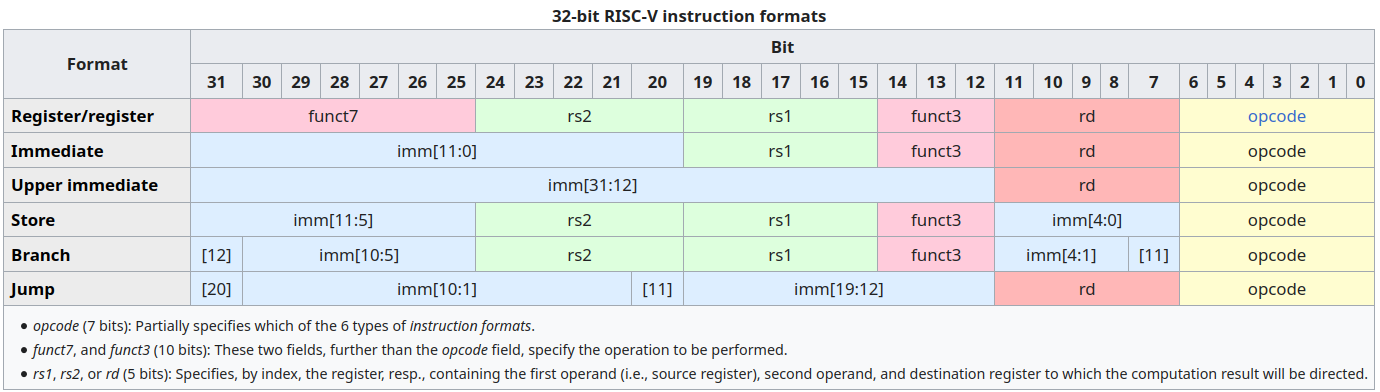
\includegraphics[width=1\linewidth]{img/\jobname/RISCV_instruction_format_wikipedia}
    \end{figure}

    \begin{itemize}
        \tightlist
        \item \textbf{Reg/reg} операции над несколькими регистрами \\
        \mintinline{c}{s0 = s1 + s2;} $\rightarrow$ \mintinline{gas}{add s0, s1, s2}; или\\
        \mintinline{c}{s0 = s1;} $\rightarrow$ \mintinline{gas}{add s0, s1, zero}
        \item \textbf{Immediate} операция над регистром и константой \\
        \mintinline{c}{s0 = s1 - 12;} $\rightarrow$ \mintinline{gas}{addi s0, s1, -12}
        \item \textbf{Upper immediate} загрузка константы в старшие биты регистра\\
        \mintinline{c}{s2 = 0xABCDE123;} $\rightarrow$ \\
        $\rightarrow$ \mintinline{gas}{lui s2, 0xABCDE} \\
        {\color{white} $\rightarrow$} \mintinline{gas}{addi s2, s2, 0x123}
    \end{itemize}
\end{frame}

\begin{frame}[fragile]{Формат машинного кода и примеры команд (4, 5)}
    \begin{figure}
        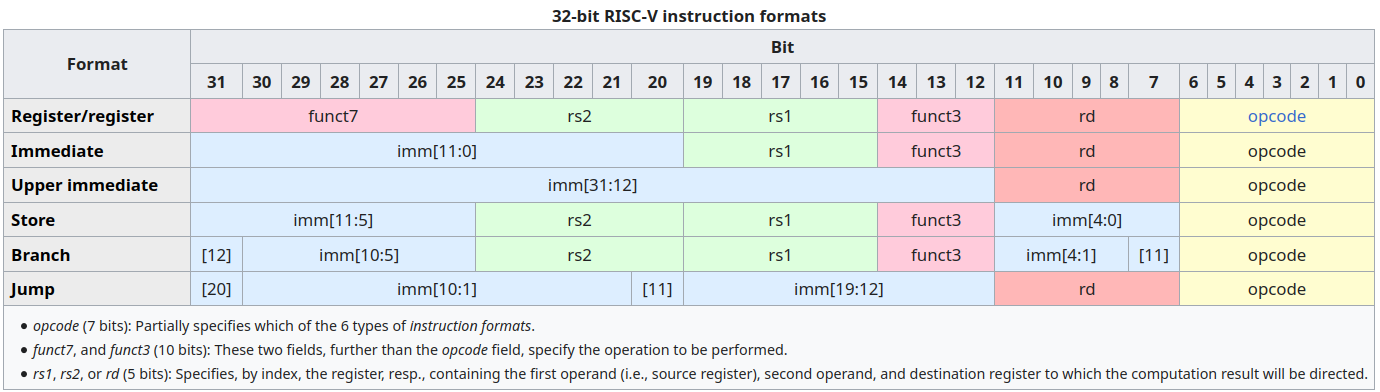
\includegraphics[width=1\linewidth]{img/\jobname/RISCV_instruction_format_wikipedia}
    \end{figure}

    \begin{itemize}
        \tightlist
        \item \textbf{[Load]/Store} операция с короткими индексами массивов\\
        \mintinline{c}{char a[10]; s2 = a[5];} $\rightarrow$ \\
        $\rightarrow$ \mintinline{text}{загр адр. a в t1} \\
        {\color{white}$\rightarrow$} \mintinline{gas}{lb t5, 5(t1)}
        \item \textbf{Branch} ветвление или безусловный переход\\
        \mintinline{c}{if(s1 >= t2) goto недалеко; } $\rightarrow$
        \mintinline{gas}{bge s1, t2, недалеко}\\
        \mintinline{c}{goto недалеко;} $\rightarrow$
        \mintinline{gas}{beq zero, zero, недалеко} (можно и проще, ниже)\\
        (недалеко --- адрес относительный)
    \end{itemize}
\end{frame}

\begin{frame}[fragile]{Формат машинного кода и примеры команд (6)}
    \begin{figure}
        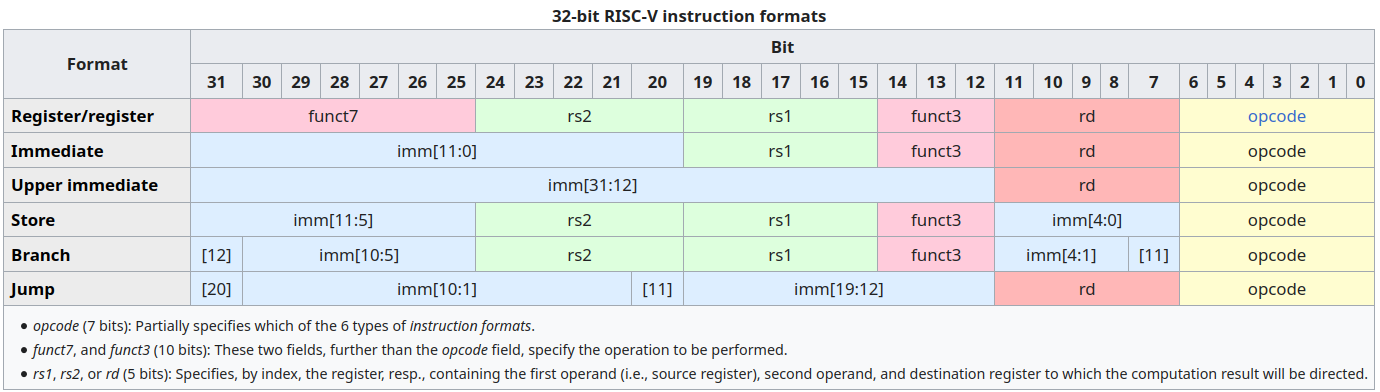
\includegraphics[width=1\linewidth]{img/\jobname/RISCV_instruction_format_wikipedia}
    \end{figure}

    \begin{itemize}
        \tightlist
        \item \textbf{Jump} --- вызов, т.е. переход с сохранением адреса возврата\\
        \begin{minted}{c}
            void leaf(){}
            int main(){leaf(); return 0;}
        \end{minted}
        $\rightarrow$ \mintinline{gas}{jal ra, leaf}\\
        Но так сделать и безусловный переход: \mintinline{gas}{j недалеко} $\leftrightarrow$ \mintinline{gas}{jal zero, недалеко}
        \item Снова \textbf{Immediate} --- возврат из функции \\
        возврат \mintinline{gas}{ret} на самом деле \mintinline{gas}{jalr zero, ra, 0} --- перейти по
        адресу в \mintinline{gas}{ra + 0}, исходный адрес записать в \mintinline{gas}{zero} (выкинуть)
    \end{itemize}
\end{frame}

\begin{frame}{Общее впечатление от системы команд}
    \begin{outline}[itemize]
        \1 Язык всё ещё не для человека:
            \2 загрузка длинных констант в два захода
            \2 «не очевидная» (но удобная для электроники!) мешанина с командами вызова и перехода
        \1 Машинный код действительно простой!
        \1 Благодаря регистру \mintinline{gas}{zero} из «странных» команд делаются более очевидные «псевдокоманды»:
            \2 \mintinline{gas}{jalr zero, ra, 0} $\rightarrow$ \mintinline{gas}{ret}
            \2 \mintinline{gas}{jal zero, недалеко} $\rightarrow$ \mintinline{gas}{j недалеко}
            \2 \mintinline{gas}{sub s1, zero, s0} $\rightarrow$ \mintinline{gas}{neg s1, s0} $\leftrightarrow$ \mintinline{c}{s1 = -s0}
            \2 \mintinline{gas}{addi x0, x0, 0} $\rightarrow$ \mintinline{gas}{nop}
            \2 и т.д.
    \end{outline}
    \pause
    \alert{За пределами лекции:}
    \begin{itemize}
        \item расширение C(ompact) --- формат машинного кода, в котором некоторые команды по 2 байта
        \item RISC-V 32 vs 64 --- у RISC-V 64 регистры 64-битные, но машинный код 32-битный
    \end{itemize}

\end{frame}

\subsection{Конвейер}

\begin{frame}{Конвейер}
    Наличие и характер конвейера зависит от реализации
    \pause
    \begin{block}{Конвейер распознаёт конфликты}
        Потому что реализации стремятся быть (и являются) достаточно умными, и поддерживать:
        \begin{itemize}
            \tightlist
            \item Суперскалярность
            \item Предсказание переходов
            \item В пределе --- внеочередное исполнение
        \end{itemize}
        Т.е. у конвейера нет шансов остаться таким же простым, как и у MIPS
    \end{block}
    \pause
    \href{https://stackoverflow.com/a/54725021}{Обсуждение на Stack Overflow}
\end{frame}

\subsection{Кросс-компиляция}

\begin{frame}{Кросс-компиляция}
    \begin{itemize}
        \item При помощи \href{https://buildroot.org/}{BuildRoot}
        \item С отладкой — при помощи \href{http://ripes.me/Ripes/}{Ripes} %или \href{http://ripes.me/}{Онлайнового} Ripes
    \end{itemize}
\end{frame}

%==============================================

\section*{}

\begin{frame}{Вопросы и упражнения}
    \begin{block}{Вопросы}
        \begin{enumerate}
            \tightlist
            \item
            Расскажите о составе регистрового файла x86
            \item
            Расскажите о составе регистрового файла RISC-V
            \item
            Приведите примеры арифметико-логических команд x86
            \item
            Приведите примеры арифметико-логических команд RISC-V
            \item
            Что такое микроциклы x86?
            \item
            Приведите примеры и опишите работу нескольких команд условного
            перехода x86
            \item
            Приведите примеры и опишите работу нескольких команд условного
            перехода RISC-V
        \end{enumerate}
    \end{block}

    \begin{block}{Упражнения}
        \begin{enumerate}
            \tightlist
            \item
            Скомпилируйте программу из примера для любой незнакомой архитектуры;
            пользуясь справочниками, объясните действия всех машинных команд
        \end{enumerate}
    \end{block}
\end{frame}

\postamble

\end{document}
